% 
\documentclass{beamer}          % works better for video meetings.
% NOT \documentclass[aspectratio=169]{beamer}
\usepackage{graphicx}
\usepackage{hyperref}
\usepackage{verbatim}
\usepackage{xcolor} % to access the named colour LightGray
\definecolor{LightGray}{gray}{0.9}
\usepackage{minted}
\usemintedstyle{vs}
\usepackage{amsmath}
\usepackage{unicode-math}
%\setbeamertemplate{itemize item}{\color{SpOrange}}
%    \setbeamertemplate{itemize subitem}{\color{SpOrange}}
%%% Below imports didnt work
%\usepackage{newunicodechar}
%\usepackage{jlcode}
%\usepackage{fontspec}
%\usepackage{polyglossia}
%\setmonofont{DejaVu Sans Mono}[Scale=MatchLowercase]
%\usepackage[T1]{fontenc}
%\usepackage{times}

% Logo insertion ideas from
% https://latex-beamer.com/tutorials/logo-beamer/

%\usetheme{AnnArbor}
\usecolortheme{XKDR}
\logo{
\includegraphics[width=0.8cm]{./XKDR_Logomark_RGB_Full_Colour.png}}

\hypersetup{colorlinks,
    citecolor=blue,
    linkcolor=blue,
    }

\mode<presentation>
{
  \usetheme{boxes}
}

\usepackage[english]{babel}
\usepackage[utf8]{inputenc}

% Or whatever. Note that the encoding and the font should match. If T1
% does not look nice, try deleting the line with the fontenc.

\newcommand{\fullpage}[1]{
  \begin{frame}
    \vfill
    {\Large #1}
    \vfill
  \end{frame}
}

\addtobeamertemplate{navigation symbols}{}{%
    \usebeamerfont{footline}%
    \usebeamercolor[fg]{footline}%
    \hspace{1em}%
    {\large \insertframenumber/\inserttotalframenumber}
}

\title{Surveys with Julia}
\subtitle{Introduction to Survey.jl}
% \titlegraphic{
\includegraphics[width=2.88cm]{./XKDR_Primary_Logo_RGB_Full_Colour.png}}
\titlegraphic{
\includegraphics[width=2.4cm]{./XKDR_Primary_Logo_RGB_Full_Colour.png}}

%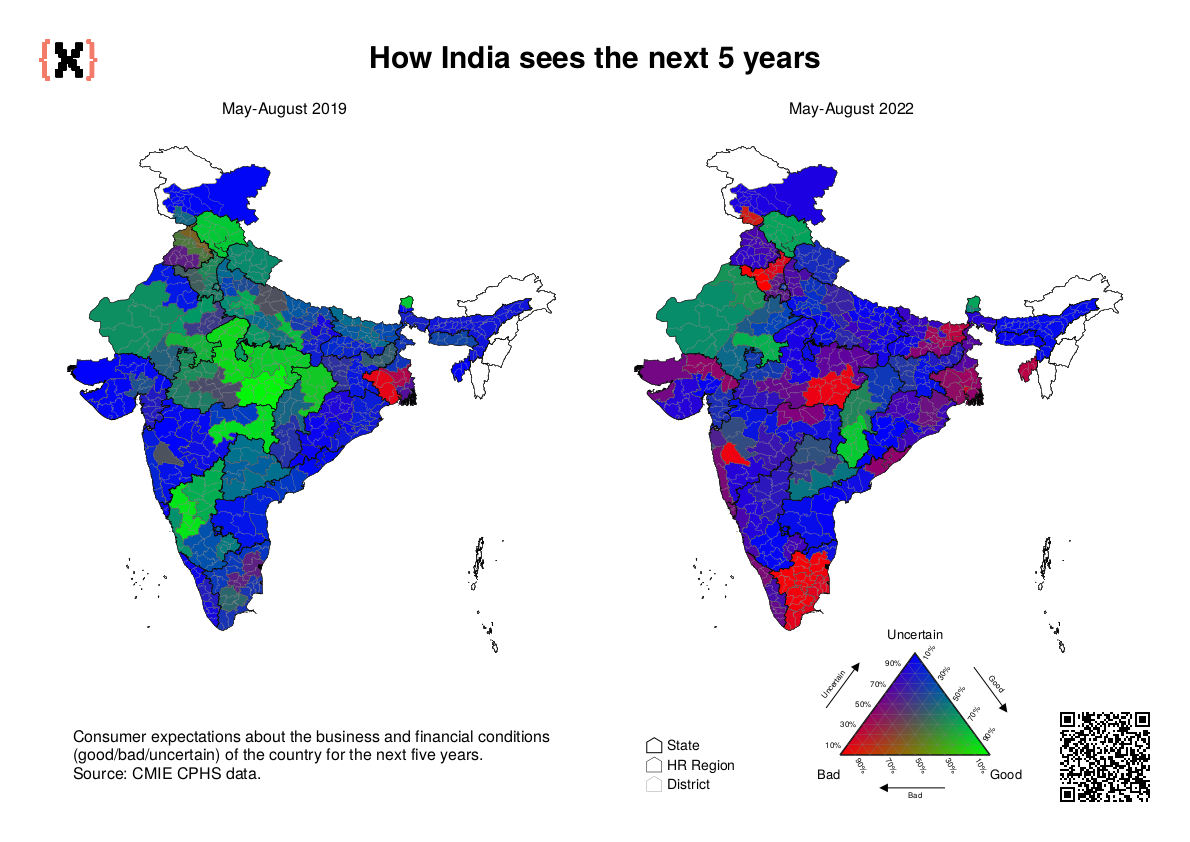
\includegraphics{survey_maps.png}

\author{Shikhar Mishra}

\hypersetup{pdfauthor   = XKDR Forum https://xkdr.org,
            pdftitle    = Surveys with Julia,
            pdfsubject  = Survey.jl introduction, 
            pdfkeywords = {surveys, India, research organisations, XKDR Forum}
}

\begin{document}

\begin{frame}
  \titlepage
\end{frame}

\begin{frame}
  \frametitle{What is complex survey analysis?}
  \begin{columns}
           \column{0.65\linewidth}
           
  \begin{itemize}
  
  \item Surveys are an empirical tool for social and behavioural analysis
  \item \textbf{Goal:} obtaining estimates for a large population by surveying a well selected subset
  \item In contrast to a \textbf{census}
  \item Techniques available for increasing \underline{precision} and \underline{representation} of the survey
   	\begin{itemize}
  		\item Several types of survey "designs" and sampling methods
  	\end{itemize} 
	\end{itemize}
	
	\column{0.3\linewidth}
	\centering
	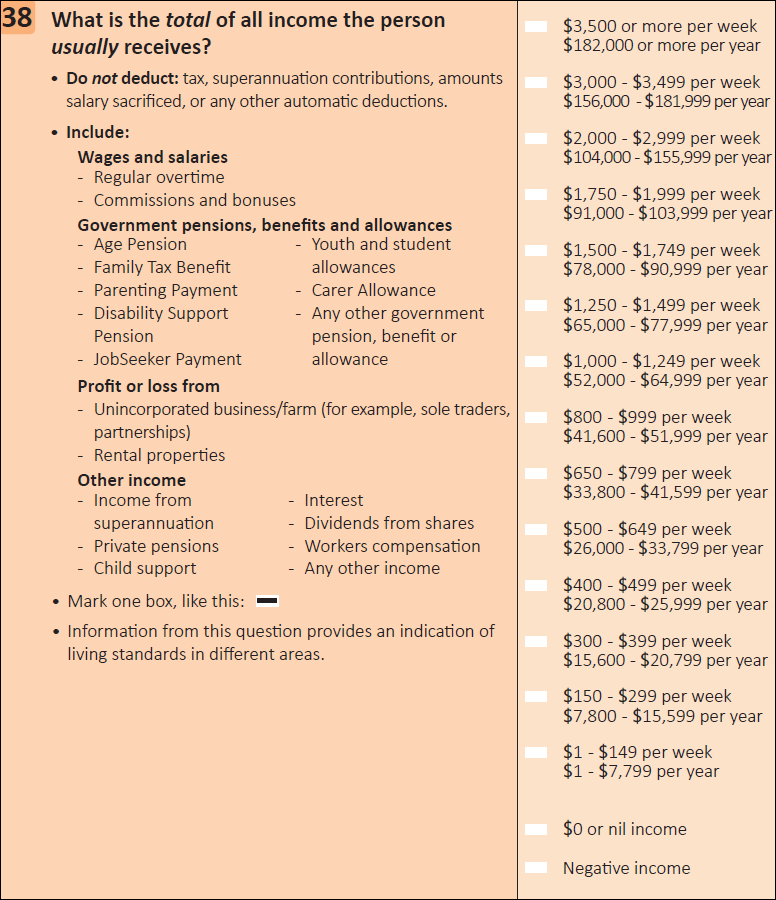
\includegraphics[height=5cm, width=3.5cm]{Q38}
\end{columns}
\end{frame}

\begin{frame}{Some survey terminology}
    \begin{description}
    \item[Weighting] How many people does each respondent represent?
    \item[Strata] Subgroups of the population known a priori eg. states, districts, gender. Strata info used to improve representation
    %NOTE: Works best when population is homogeneous within strata, and different across strata.
    \item[Clusters] Logistical constraints on survey sampling, can only visit $n$ states, districts and suburbs
    \end{description}
\end{frame}

\begin{frame}{Why does a "survey analysis" package do?}  
	\begin{itemize}
	\item Computing summary statistics from a survey requires  applying mathematical corrections and adjustments
  	\begin{itemize}
  		\item eg. population mean is not as simple as arithmetic mean of a numeric vector
%  		\item Estimates "grouped by" a demographic variable require
  	\end{itemize}
  	\item Point estimation (relatively) easy
  	\item Variance estimation is complex
  	\item A "survey" package:
  	\begin{itemize}
  		\item exposes an intuitive API to user
  		\item automatically applies formulae and corrections in background
  	\end{itemize}
  	\item Eg. in Survey.jl for population mean (with SE) of a variable you can do \texttt{mean(:variable,data)}
	\end{itemize}
\end{frame}

\begin{frame}{Our engineering journey}
\begin{itemize}
  \item Users of R \texttt{survey} package
  	\begin{itemize}
  		\item Benchmark for open-source complex survey analysis
  		\item CMIE CPHS, Prowess, NFHS etc
  	\end{itemize}	
  \item R `survey` designed in early 2000's for MB's of data 
	\begin{itemize}
  		\item slow for "large" modern datasets and many class of simulation problems
  		\item eg. variance estimation using bootstrapping
  		\item Computation times upto few hours for simple summary statistics
   	\end{itemize}
   	\item Real-world performance a key factor in development of \texttt{Survey.jl}
\end{itemize}
\end{frame}

\begin{frame}{Why Julia for complex survey analysis}
	\begin{description}
		\item[Performance]  \textbf{Expressivity} of R/Python meets \textbf{speed}  of a systems language
		\item[Development] Avoid "two-language problem". Survey researchers just want something that works great out of the box. Easy maintenance.
		\item[Community] Several unmaterialised attempts to create survey analysis package. We received feedback and even contributing PRs.\hyperlink{appendix_end}{\beamergotobutton{1}} 
		\item[Ecosystem] Julia has substantial statistical computing abilities, with state of the art \texttt{DataFrames, Makie, Optim, Turing, Flux, LinearAlgebra} packages. \\ \texttt{Survey} is complement to and complemented by the entire data ecosystem.
	\end{description}			
\end{frame}

\begin{frame}{Survey.jl}  
  An efficient computing framework for survey analysis\\
%  \\ \\ \textbf{Features}
  \begin{itemize}
  \item Summary statistics - \texttt{mean}, \texttt{total}, \texttt{ratio}, and \texttt{quantile}
  \item Subpopulations / domain estimation for subsets of sample
  \item Variance estimation using (Rao-Wu) bootstrap
  \begin{itemize}
    \item 1000 MC simulations for variance in Julia takes similar computation time as 50 simulations in R.
  \end{itemize}
  \item Modularity - Can write custom replicate weighting algorithm
  \item Visualisations support for weighted scatter plots, histograms
  \item Tested and compared against R \texttt{survey}
   \end{itemize}
\end{frame}

\begin{frame}{Survey.jl}
	Getting started with Survey.jl
	\href{https://github.com/xKDR/Survey.jl}{GitHub} and \href{https://xkdr.github.io/Survey.jl/dev/}{Documentation}
\end{frame}

\begin{frame}[fragile]{Demo workflow}
\framesubtitle{Import and load data}
\textbf{Survey:} CMIE Consumer Pyramids Household Survey - Multistage stratified high frequency survey of Indian households
\scriptsize
\begin{minted}[breaklines,escapeinside=||,mathescape=true, linenos, numbersep=3pt, frame=lines, fontsize=\small, framesep=2mm]{julia}
# Imports and housekeeping
...
# Connect to SQL server
conn = DBInterface.connect(MySQL.Connection, host, user, password; db = "hhd")
query = "SELECT RESPONSE_STATUS, STATE, HR, DISTRICT, STRATUM, PSU_ID, REGION_TYPE, FAMILY_SHIFTED, HH_ID, MONTH_SLOT, MONTH, TOTAL_INCOME , HH_WEIGHT_MS, HH_NON_RESPONSE_MS  FROM hh_income_monthly WHERE MONTH = 'Apr 2022' AND RESPONSE_STATUS = 'Accepted'"
# Pipe query output into DataFrame
df = DBInterface.execute(conn, query) |> DataFrame
\end{minted}
\end{frame}

\begin{frame}[fragile]{Demo workflow}
\framesubtitle{Create SurveyDesign}
\begin{minted}[breaklines,escapeinside=||,mathescape=true, numbersep=3pt, frame=lines, fontsize=\small, framesep=2mm]{julia}
# Load df into survey design object
julia> CPHS_income = SurveyDesign(df, clusters = :HH_ID, strata = :STRATUM, weights = :HH_WEIGHT_MS)

SurveyDesign:
data: 123816×17 DataFrame
strata: STRATUM
    [HR 1_URBAN_S, HR 1_URBAN_S,  …  HR 110_RURAL_R]
cluster: HH_ID
    [5.3877505e7, 4.3406519e7  …  6.742216e7]
popsize: [8.81791619977e7  …  1.034108342135e8]
sampsize: [123816, 123816, 123816  …  123816]
weights: [712.1791, 712.1791, 712.1791  …  835.1977]
allprobs: [0.0014, 0.0014, 0.0014  …  0.0012]
\end{minted}
\end{frame}

\begin{frame}[fragile]{Demo workflow}
\framesubtitle{Create ReplicateDesign}
%\scriptsize
\begin{minted}[breaklines,escapeinside=||,mathescape=true, numbersep=3pt, frame=lines, fontsize=\small, framesep=2mm]{julia}
# Create replicate design using Rao-Wu bootstrap weights
julia> CPHS_income_bootstrap = bootweights(CPHS_income, replicates = 500)

ReplicateDesign:
data: 123816×517 DataFrame
strata: STRATUM
    [HR 1_URBAN_S, HR 1_URBAN_S  …  HR 102_URBAN_M]
cluster: HH_ID
    [1.0034716e7, 1.0190136e7  …  9.9842237e7]
popsize: [8.81791619977e7  …  2.92096840303e7]
sampsize: [123816, 123816, 123816  …  123816]
weights: [712.1791, 712.1791, 712.1791  …  235.912]
allprobs: [0.0014, 0.0014, 0.0014  …  0.0042]
replicates: 500
\end{minted}
% NOTE: highlight 517 and 500 here and explain
\end{frame}

\begin{frame}[fragile]{Demo workflow with CPHS}
\framesubtitle{Calculate summary statistics}
\begin{minted}[breaklines,escapeinside=||,mathescape=true, numbersep=3pt, frame=lines, fontsize=\scriptsize, framesep=2mm]{julia}
# Mean income (overall India)
julia> mean(:TOTAL_INCOME, CPHS_income_bootstrap) 
1×2 DataFrame
 Row │ mean     SE      
     │ Float64  Float64 
─────┼──────────────────
   1 │ 23870.2  81.8377

# Total income by homogenous regions (Subpopulation estimation)
julia> total(:TOTAL_INCOME, :HR, CPHS_income_bootstrap)
102×3 DataFrame
 Row │ HR       total       SE        
     │ String   Float64     Float64   
─────┼────────────────────────────────
   1 │ HR 1     3.95686e10  6.88132e8
   2 │ HR 2     6.72443e9   1.96195e8
   3 │ HR 3     1.93887e10  6.04332e8
  ⋮  │    ⋮         ⋮           ⋮
 101 │ HR 95    1.4761e10   4.65155e8
 102 │ HR 97    1.83399e10  3.58032e8
                       93 rows omitted
\end{minted}
\end{frame}

%\begin{frame}[fragile]{Demo workflow with CPHS}
%\begin{minted}[breaklines,escapeinside=||,mathescape=true, numbersep=3pt, frame=lines, fontsize=\scriptsize, framesep=2mm]{julia}
%@benchmark bootweights(CPHS, replicates = 500) samples = 10
%@benchmark  samples = 10
%@benchmark mean(:TOTAL_INCOME, :HR, CPHS_bootstrap) samples = 1
%\end{minted}
%\end{frame}


\begin{frame}{Plans}
	Efficient implementations of all the methods in R `survey`. Features for future releases will include:
	\begin{itemize}
		\item Proportion and count estimation
		\item Variance by Taylor linearization for `SurveyDesign`
		\item More replicate weighting algorithms (BRR, Jackknife, other types of bootstrap) for `ReplicateDesign`
		\item Post-stratification, raking, calibration, GREG estimation
		\item Frequency/contingency table analysis, association tests
		\item Missing data handling (like R \href{https://cran.r-project.org/web/packages/mitools/index.html}{mitools})
		\item Integration with survival analysis tools
		\item Integration with \href{https://github.com/JuliaStats/GLM.jl}{GLM.jl}
		\item Out-of-memory integration with SQL databases
	\end{itemize}
\end{frame}

\begin{frame}{Credits}
	We gratefully acknowledge the \href{https://julia.mit.edu}{JuliaLab} at MIT for financial support for this project. \\ \\
	\textbf{Contributors:} \\
	\begin{itemize}
	\item \href{https://github.com/ayushpatnaikgit}{Ayush Patnaik}, XKDR and U Sydney
	\item \href{https://github.com/smishr}{Shikhar Mishra} XKDR and ANU
	\item \href{https://github.com/iuliadmtru}{Iulia Dmitru}, GSoc and XKDR, U Bucharest, Romania
	\item \href{https://github.com/codetalker7}{Siddhant Chaudhary}, Chennai Maths Institute (CMI)
	\item \href{https://github.com/sayantikaSSG}{Sayantika Sengupta}, CMI
	\item \href{https://github.com/nadiaenh}{Nadia Enhaili}, UBC Vancouver
	\item \href{https://github.com/greimel}{Fabian Greimel} Asso Prof of Economics, U Amsterdam
	\end{itemize}
\end{frame}

%\begin{frame}{Credits}
%	We gratefully acknowledge the JuliaLab at MIT for financial support for this project.
%\end{frame}

\appendix

\begin{frame}[label=appendix_end]{References}
  \begin{itemize}
  	\item \href{https://www.amazon.com/Assisted-Survey-Sampling-Springer-Statistics/dp/0387406204}{Model Assisted Survey Sampling} (1992)
  	\item \href{https://www.routledge.com/Sampling-Design-and-Analysis/Lohr/p/book/9780367279509}{Sampling: Design and Analysis}, Sharon Lohr, (2010)	
  	\item \href{https://journals.sagepub.com/doi/10.1177/096228029600500305}{JNK Variance Estimation Literature Review}

  	\item R survey package \href{https://r-survey.r-forge.r-project.org/survey/}{documentation}  	
  	\item Julia Discourse posts \href{https://discourse.julialang.org/t/any-package-for-survey-data-analysis/67317}{here} and \href{https://discourse.julialang.org/t/analysis-of-complex-surveys-in-julia/44011}{here}
  	\item Unmaterialised attempts \href{https://github.com/samplics-org/survey.jl}{samplics/survey.jl} and \href{https://github.com/jamanrique/SurveyAnalysis.jl}{jamanrique/SurveyAnalysis.jl}
\end{itemize}
\end{frame}

\end{document}

%  	\item SAS Survey PROCS \href{https://support.sas.com/rnd/app/stat/procedures/SurveyAnalysis.html#surveymeans}{documentation}

%    \item[] Now you can make it clear you've done a shitload of work
%      \begin{itemize}
%      \item[]  without having to show everything! \hyperlink{appendix_start}{\beamergotobutton{Back}}
%      \end{itemize}
%    \item[] You label a frame with the \texttt{[label=name]} option, and then point a link to it
%    \item[] You can make an object a link using the \texttt{\textbackslash hyperlink\{label\}\{object\}} command


%\begin{frame}
%  \hfill {\LARGE Thank you}.
%
%  \vfill
%  \vfill
%
%  \hfill \url{https://xkdr.org}
%\end{frame}
